	\documentclass[../pfc.tex]{subfiles}
	
	\begin{document}
	
	\section{Plan de desarrollo de software}
	
	Para el desarrollo de este aplicativo se seguirán los principios del Agile Manifesto \cite{agile}, y de entre todas las metodologías que lo implementan utilizaremos Scrum, ya que nos permite desarrollar siempre sobre algo ejecutable y tiene una buena "pelea contra el tiempo" o "timeboxing" ya que al final de cada sprint hay que hacer una retrospectiva sobre lo que ya se ha construido y entregado.

	\section{Propósito general de la planificación}
	
	La planificación nos debe dar una cifra orientativa del esfuerzo a comprometer para acometer un desarrollo de un proyecto software. Pero debido a lo mencionado anteriormente sobre el manifiesto ágil, creemos que dar una cifra estimativa en tiempo es venturoso, más si queremos ceñirnos a el y más aún cuanto mas a largo plazo sea la estimación. Por eso las metodologías ágiles suelen ocultar la referencia temporal de los desarrollos y estiman la complejidad de las tareas, sabiendo por el histórico, ya que los equipos deben ser fijos en el tiempo, la complejidad aproximada que un equipo dedicado a un proyecto puede acometer. 
	
	\section{Metodología }
	
	Para la realización del proyecto, dentro las diferentes metodologías ágiles, hemos elegido SCRUM, por ser la que mejor se adapta a la continua pelea contra el tiempo que el equipo debe mantener. \\
	Lo primero que debemos decir es que SCRUM es una metodología iterativa e incremental que promueve la auto organización de los equipos de desarrollo y un esquema de colaboración con el cliente, haciéndose responsable de que las prioridades, los requisitos, etc pueden cambiar por parte de este, y que es responsabilidad del propio equipo el asumir y responder a estos cambios. 
	
	\subsection{SCRUM}
	
	SCRUM como metodología fué propuesto por Ikujiro Nonaka e Hirotaka Takeuchi a principios de los 80, al analizar cómo desarrollaban los nuevos productos las principales empresas de manufactura tecnológica: Fuji-Xerox, Canon, Honda, Nec, Epson, Brother, 3M y Hewlett-Packard (Nonaka \& Takeuchi, The New New Product Development Game, 1986).\\
	Aunque esta forma de trabajo surgió en empresas de productos tecnológicos, es apropiada para proyectos con requisitos inestables y para los que requieren rapidez y flexibilidad, situaciones frecuentes en el desarrollo de determinados sistemas de software.\\
	
	SCRUM define un conjunto de prácticas y roles, que pueden tomarse como punto de partida para definir el proceso de desarrollo que se ejecutará durante un proyecto. Abordar un proyecto mediante SCRUM lleva a la repetición o iteración de la unidad básica del peoyecto denominada Sprint. Durante cada sprint, un periodo entre una y cuatro semanas (la magnitud es definida por el equipo y debe ser lo mas corta posible), el equipo crea un incremento de software potencialmente entregable (utilizable). El conjunto de características que forma parte de cada sprint viene del Product Backlog, que es un conjunto de requisitos de alto nivel priorizados que definen el trabajo a realizar a menudo denominadas Historias de usuario. Los elementos del Product Backlog que forman parte del sprint se determinan durante la reunión de Sprint Planning. Durante esta reunión, el Product Owner identifica los elementos del Product Backlog que quiere ver completados y los hace del conocimiento del equipo. Entonces, el equipo conversa con el Product Owner buscando claridad y magnitud adecuadas para luego determinar la cantidad de ese trabajo que puede comprometerse a completar durante el siguiente sprint. Durante el sprint, nadie puede cambiar el Sprint Backlog, lo que significa que los requisitos del sprint están congelados durante el propio sprint, pero podrían modificarse aquellos que aun estuviesen en el Product Backlog.\\
	
	SCRUM permite la creación de equipos autoorganizados impulsando la co-localización de todos los miembros del equipo, y la comunicación verbal entre todos los miembros y disciplinas involucrados en el proyecto, ya que una de la bases de SCRUM en la colaboración y comunicación entre todos los roles de un proyecto. \\
	
	Un principio clave de SCRUM es el reconocimiento de que durante un proyecto los clientes pueden cambiar de idea sobre lo que quieren y necesitan, y que los desafíos impredecibles no pueden ser fácilmente enfrentados de una forma predictiva y planificada. Por lo tanto, SCRUM adopta una aproximación pragmática, aceptando que el problema no puede ser completamente entendido o definido, y centrándose en maximizar la capacidad del equipo de entregar rápidamente y responder a requisitos emergentes.\\
	
	Las características más marcadas que se logran notar en SCRUM serían: gestión regular de las expectativas del cliente, resultados anticipados, flexibilidad y adaptación, retorno de inversión, mitigación de riesgos, productividad y calidad, alineamiento entre cliente y equipo, por último equipo motivado. Cada uno de estos puntos mencionados hacen que el SCRUM sea utilizado de manera regular en un conjunto de buenas prácticas para el trabajo en equipo y de esa manera obtener resultados posibles.\\
	
	Los beneficios para las empresas más notables al utilizar SCRUM son
	
	\begin{itemize} 
		\item Flexibilidad a cambios. Gran capacidad de reacción ante los cambiantes requerimientos generados por las necesidades del cliente o la evolución del mercado. El marco de trabajo está diseñado para adecuarse a las nuevas exigencias que implican proyectos complejos.
		Reducción del Time to Market. El cliente puede empezar a utilizar las características más importantes del proyecto antes de que esté completamente terminado. 
		\item Mayor calidad del software. El trabajo metódico y la necesidad de obtener una versión de trabajo funcional después de cada iteración, ayuda a la obtención de un software de alta calidad.
		Mayor productividad. Se logra, entre otras razones, debido a la eliminación de la burocracia y la motivación del equipo proporcionado por el hecho de que pueden estructurarse de manera autónoma.
		\item Maximiza el retorno de la inversión (ROI). Creación de software solamente con las prestaciones que contribuyen a un mayor valor de negocio gracias a la priorización por retorno de inversión.
		\item Predicciones de tiempos. A través de este marco de trabajo se conoce la velocidad media del equipo por sprint, con lo que es posible estimar de manera fácil cuando se podrá hacer uso de una determinada funcionalidad que todavía está en el Backlog.
		\item Reducción de riesgos El hecho de llevar a cabo las funcionalidades de mayor valor en primer lugar y de saber la velocidad a la que el equipo avanza en el proyecto, permite despejar riesgos efectivamente de manera anticipada
	\end{itemize}
	
	Aunque más adelante en este documento se profundiza en la metodología aquí se muestra una imagen que puede servir como resumen de todos los conceptos roles y rituales de SCRUM.
	
		\begin{figure}[h]
			\centering
			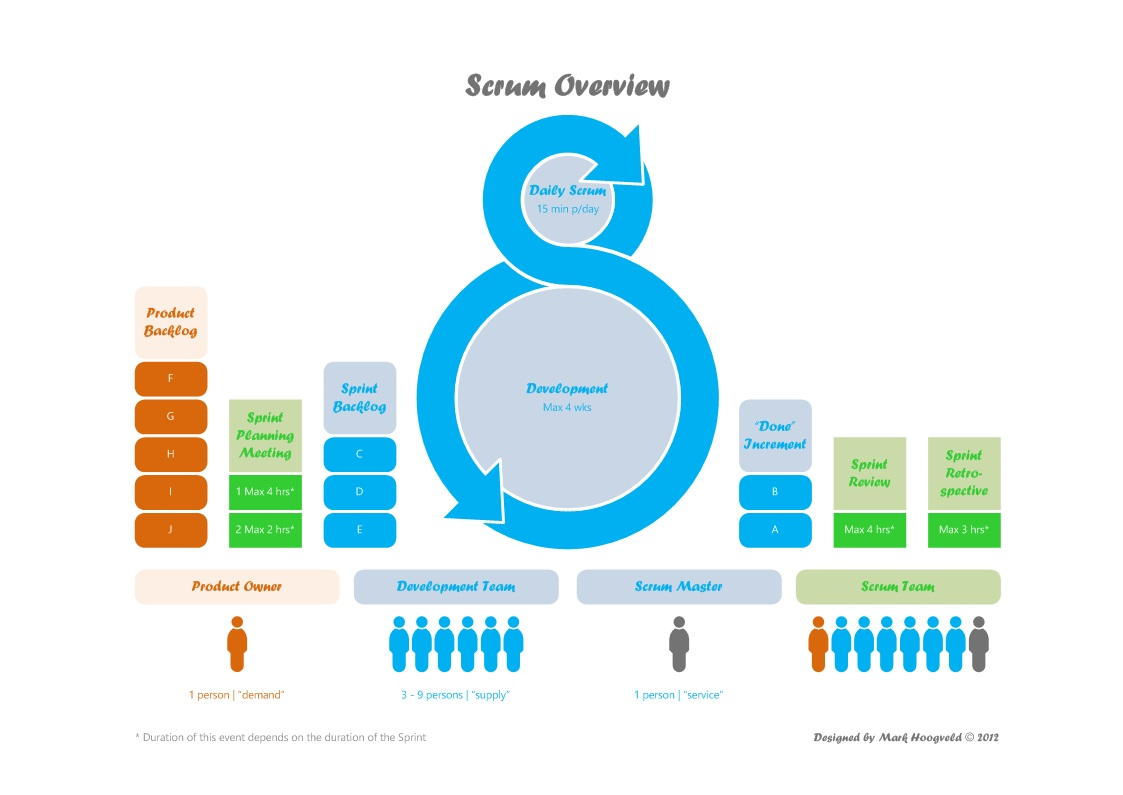
\includegraphics[max width=\textwidth]{scrum-overview}
			\caption{Resumen de Scrum.}
			\label{fig:Resumen de Scrum}
		\end{figure}
	
	\subsection{Roles y responsabilidades}
	Los roles  implicados en el proceso de desarrollo y sus responsabilidades   de la app son:

	\textbf{Product Owner}\\*
	El Product Owner representa la voz del cliente, que puede ser el cliente mismo o alguien en su nombre. Se asegura de que el equipo trabaje de forma adecuada desde la perspectiva del negocio. El Product Owner escribe historias de usuario, las prioriza, y las coloca en el Product Backlog, de hecho se suele decir que el Product Owner es el dueño del Product Backlog. E nuestro caso este rol lo llevaban a cabo varias personas con las que hemos tenido contacto en la AECC.\\
	
	\textbf{ScrumMaster (o Facilitador)}\\*
	El Scrum es facilitado por un ScrumMaster, cuyo trabajo primario es eliminar los obstáculos que impiden que el equipo alcance el objetivo del sprint. El ScrumMaster no es el líder del equipo (porque ellos se auto-organizan), sino que actúa como una protección entre el equipo y cualquier influencia que le distraiga. El ScrumMaster se asegura de que el proceso Scrum se utiliza como es debido. El ScrumMaster es el que hace que las reglas se cumplan. Quizá este es el puesto clave de Scrum ya que se encarga de que el equipo se centre en producir aquello que el Prodcut Owner ha marcado. En nuestro caso este rol ha sido una surte de Frankestein ya que para algunas tareas ha sido el personal de la AECC, para otras ha sido el tutor y en algún caso nosotros mismos saliendo del rol de equipo. \\
	
	\textbf{Equipo de desarrollo}\\*
	El equipo tiene la responsabilidad de entregar el producto. Es recomendable un pequeño equipo de 3 a 9 personas con las habilidades transversales necesarias para realizar el trabajo (análisis, diseño, desarrollo, pruebas, documentación, etc).\\
	
	A veces se definen más roles que pueden complementar en alguna fase a estos, o ayudar en tareas administrativas, pero formalmente quedan un poco fuera de la metodología por mas que sean muy necesarios en las empresas hoy día.
	
	\subsection{Eventos y rituales}
		
	\textbf{Sprint}\\* 
	El Sprint es el período en el cual se lleva a cabo el trabajo en sí. Es recomendado que la duración de los sprints sea constante y definida por el equipo con base en su propia experiencia. Se puede comenzar con una duración de sprint en particular (2 o 3 semanas) e ir ajustándolo con base en el ritmo del equipo, aunque sin relajarlo demasiado. Al final de cada sprint, el equipo deberá presentar los avances logrados, y el resultado obtenido es un producto potencialmente entregable al cliente. Asimismo, se recomienda no agregar objetivos al sprint o sprint backlog a menos que la falta de estos objetivos amenace al éxito del proyecto. La constancia permite la concentración y mejora la productividad del equipo de trabajo.\\
	
	\textbf{Daily Scrum o Stand-up meeting}\\*
	Cada día de un sprint, se realiza la reunión sobre el estado de un proyecto. Esto se llama daily standup o Stand-up meeting. El scrum tiene unas guías específicas:
	\begin{itemize} 
		\item La reunión comienza puntualmente a su hora. 
		\item Todos son bienvenidos, pero sólo los involucrados en el proyecto pueden hablar. (Esto es el equipo y el scrum master). 
		\item La reunión tiene una duración fija de 15 minutos, de forma independiente del tamaño del equipo.
		\item La reunión debe ocurrir en la misma ubicación y a la misma hora todos los días.
		\item Durante la reunión, cada miembro del equipo contesta a tres preguntas:
		\begin{enumerate}
			\item ¿Qué has hecho desde ayer?
			\item ¿Qué es lo que harás para mañana?
			\item ¿Has tenido algún problema que te haya impedido alcanzar tu objetivo? (Es el papel del ScrumMaster recordar y anotar estos impedimentos para su posterior análisis y subsanación si procede).
		\end{enumerate} 
	\end{itemize}
	
	\textbf{Reunión de Planificación del Sprint }\\*
	Al inicio de cada ciclo de Sprint, se lleva a cabo una reunión de planificación del Sprint. en esta reunión debe estar el equipo al completo, el scrum master y el product owner Se pretende:
	\begin{itemize} 
		\item Seleccionar qué trabajo se llevará a cabo por el equipo durante el sprint 
		\item Preparar, con el equipo completo, el Sprint Backlog o sea las tareas del sprint clarificando el Product Owner las posibles dudas o  inconsistencias que el equipo detecte en la redacción de las tareas, este se debe extraer de las tareas más prioritarias del Product Backlog, de acuerdo con el Product Owner. 
		\item Identificar y comunicar cuánto del trabajo es probable que se realice durante el actual Sprint.
	\end{itemize}
	
	Realizarse esta planificación en ocho horas como tiempo límite.\\
	
	\textbf{Reunión de Revisión del Sprint}\\*
	Al finalizar cada sprint se organiza esta reunión en la que que el equipo presenta el trabajo desarrollado durante el sprint en lo que se denomina Incremento de Producto Potencialmente Entregable. Durante esta reunión tiene lugar la presentación del ejecutable en lo que se denomina Demo. Así pues las principales actividades de esta reunión serían:
	\begin{itemize} 
		\item Revisar el trabajo que fue completado y no completado 
		\item 	Presentar el trabajo completado a los interesados, entre ellos el product owner y que estos de su aprobación al mismo o presenten sus quejas o matices (alias “demo”), pero teniendo en cuenta que los estados del trabajo son binarios, está acabado o no está acabado, no hay porcentajes intermedios. 
		\item El trabajo incompleto no puede ser demostrado 
	\end{itemize}
	
	Para esta reunión y dependiendo del tamaño del sprint se dispondrá de cuatro horas como límite\\
	
	\textbf{Retrospectiva del Sprint }\\*
	Después de cada sprint, se lleva a cabo una retrospectiva del sprint, en la cual todos los miembros del equipo dejan sus impresiones sobre el sprint recién superado. El propósito de la retrospectiva es realizar una mejora continua del proceso. Esta reunión tiene un tiempo fijo de cuatro horas.
	
	\section{Planificación completa}
	
	La planificación de la app será en puntos de historia que mediran la complejidad de la misma. Esta comlejidad será consensuada por el equipo, en la reunión "Sprint Planning" en la rutina deniominada Poker Planning.  
	
	\section{Recursos necesarios}
	
	Los recursos designados para la realización completa de este proyecto serán los siguientes:\\
	
	\textbf{Recursos humanos}
	
	- Los desarrolladores
	
	- El cliente.\\\\
	
	\textbf{Recursos Software}
	
	Los recursos software para esta iteración serán:
	
	Herramienta de planificación:
	
	- Microsoft Project 2003
	
	Herramienta de documentación:
	
	- TexStudio + Sharelatex
	
	Herramienta de ilustración
	
	- Adobe Photoshop CS6
	
	Herramienta de modelado
	
	- StarUML
	
	Herramienta de sincronización
	
	- Dropbox
	
	- GitHub
	
	Entorno integrado de desarrollo
	
	- Android Studio
	
	Entorno de Programación
	
	- Android
	
	Sistema Gestor de Bases de datos
	
	- SQLLite
	
	Otros recursos software
	
	- Notepad\\\\
	
	\textbf{Recursos Hardware}
	
	Los recursos hardware para esta iteración serán:
	
	- Dos ordenadores portátiles personales
	
	- Un ordenador Personal de sobremesa
	
	- Varios móviles con SO Android
	
	- Memoria USB para el intercambio de datos
	
	- Cables USB - Micro USB (Debug)\\\\
	
	\textbf{Otros Recursos}
	
	- Conexión a Internet \newpage
	
\end{document}